\section{Results and analysis}

\begin{figure*}[t]
\centering

\begin{tabular}{@{}
p{0.29\textwidth}
@{\hspace{0.04\textwidth}}
p{0.29\textwidth}
@{\hspace{0.04\textwidth}}
p{0.29\textwidth}
@{}}

\centering
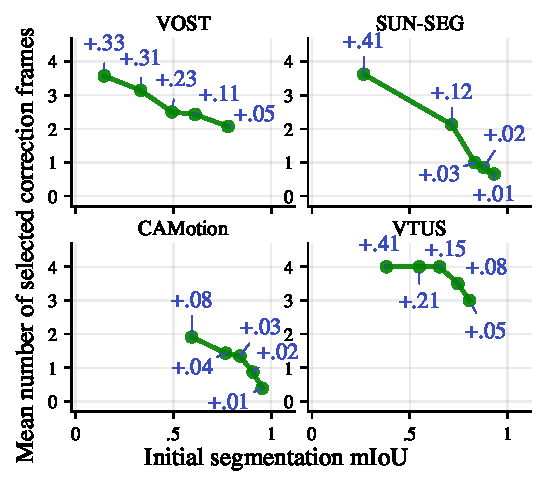
\includegraphics[width=\linewidth]
{Figures/initial_iou_vs_selected_k_binned.pdf}
\captionof{figure}{
Mean number of selected correction frames versus initial segmentation quality. Videos are grouped into five initial-mIoU bins, and the
    labels show the mean mIoU gain after correction. Lower-quality
    segmentations receive more corrections and larger gains, indicating that
    the policy allocates expert effort where it is most useful.
}
\label{fig:initial_iou_selected_k}

&

\centering
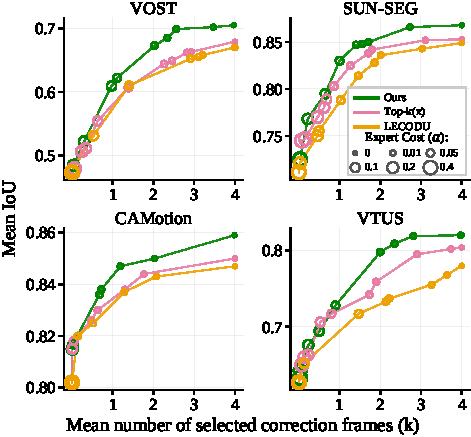
\includegraphics[width=\linewidth]
{Figures/all_datasets_iou_vs_k_expert_cost.pdf}
\captionof{figure}{
Quality--cost trade-off under varying expert-cost weight \(\alpha\).
        Each point reports the video-level mIoU and mean selected cardinality for
        one value of \(\alpha\), with marker size increasing with \(\alpha\).
        Our method is
generally above the baselines at comparable correction budgets
}
\label{fig:alpha_sweep}

&

\centering
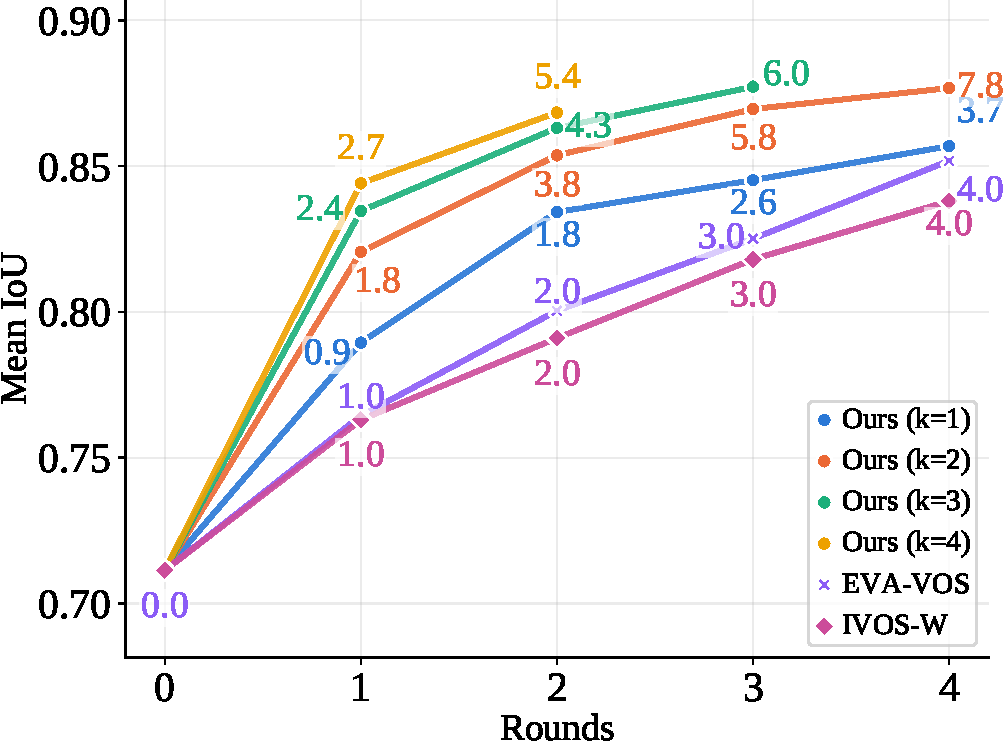
\includegraphics[width=\linewidth]
{Figures/sunseg_iterative_iou_by_iteration.pdf}
\captionof{figure}{
Mean IoU over corrective-prompting iterations on SUN-SEG at
    $\alpha=0.001$. Our models with maximum cardinality
    $K\in\{1,2,3,4\}$ select correction frames in batches, whereas EVA-VOS
    and IVOS-W select one frame per iteration. After each iteration, the
    selected frames are prompted and the video is re-propagated. Point labels
    show the cumulative number of selected frames.
}
\label{fig:sunseg_iterative_prompting}

\end{tabular}
\end{figure*}

\paragraph{Quality--cost trade-off (Q1).}

Table~\ref{tab:overall_comparison} shows that, without correction, the initial propagation yields the lowest mIoU, while random correction improves it.
L2RP requests the fewest corrections but is limited to a single frame, whereas Lazy-XMem requests $3$--$4$ corrections.
LECODU and Top-$k(x)$ incur similar system costs on CAMotion, while Top-$k(x)$ achieves lower costs on VOST, SUN-SEG and VTUS.
Our method achieves the highest mIoU with the lowest system cost.
Compared with Top-$k(x)$, ours reduces the mean cardinality by $3.1$--$9.2\%$ and the system cost by
$5.4$--$11.4\%$.
Although the oracle defines the upper bound, ours consistently remains the closest reducing $28.1$--$75.0\%$ of the
system-cost gap between Top-$k(x)$ and the oracle.

Figure~\ref{fig:coverage_curves} further shows that our method achieves the highest mIoU across non-deferral coverage levels, showing its performance gains are consistent across wide range of operating points rather than tied to a particular decision threshold.

These results show that variable-cardinality deferral improves the quality--cost trade-off by allocating correction effort according to each video, achieving higher segmentation quality without requesting more expert prompts.

\paragraph{Frame selection at fixed cardinality (Q2).}

Table~\ref{tab:fixed_cardinality} compares frame selection methods with a fixed expert budget of $k=3$.
IVOS-W and EVA-VOS perform sequential frame selection, re-propagating after each correction, whereas the batch methods select all frames in a single batch from the initial segmentation.
Despite not benefiting from intermediate propagation updates, our method achieves the highest non-oracle mIoU on all four datasets improving over EVA-VOS by $0.5$--$4.5\%$ and batch Top-$k$ by $0.6$--$4.0\%$.
Results for $k\in{1,2,3,4}$, reported in the appendix, show the same trend.

\paragraph{Allocation of expert effort (Q3).}
Figure~\ref{fig:initial_iou_selected_k} shows that the policy allocates larger correction budgets to videos with lower initial mIoU and fewer corrections to those with higher initial mIoU.
The mIoU gains are positive across all bins and are generally larger for lower-quality initial propagations.
These results indicate that the policy allocates expert effort according to both the current propagation quality and the expected benefit of additional corrections.
